\begin{Exercise}[label = boatgraph, origin = Jaan Kalda, difficulty = 4, title = Bootsbewegung]
	Die Beschleunigung eines Boots hängt von seiner Geschwindigkeit ab, wie im Bild gezeigt. Die Anfangsgeschwindigkeit des Bootes beträgt $v_0 = 4~\nicefrac{m}{s}$. Wie groß ist die Strecke, die das Boot zurücklegt hat, wenn es nahezu zum stehen kommt?
\end{Exercise}
\begin{figure}[h]
	\centering
	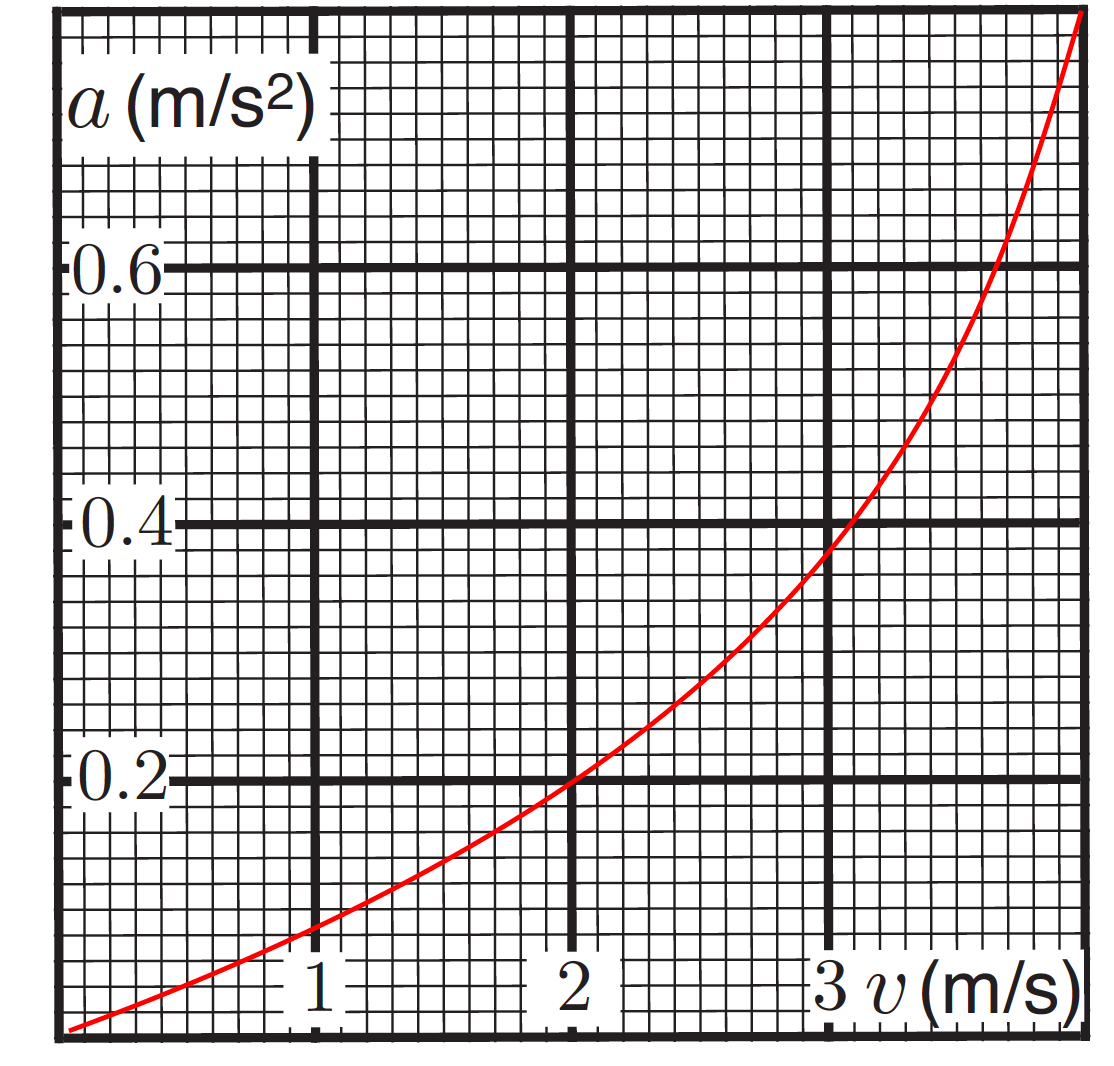
\includegraphics[scale = 0.4]{../tasks/kalda/boatgraph1}
\end{figure}